\documentclass[runningheads]{llncs}
\usepackage[T1]{fontenc}
\usepackage[utf8]{inputenc}
\usepackage[spanish,es-tabla]{babel}
\usepackage{graphicx}
\usepackage{array}
\usepackage{booktabs}
\usepackage{pdflscape}
\newcolumntype{L}[1]{>{\raggedright\arraybackslash}p{#1}}
\usepackage[hidelinks]{hyperref}

% Cabeceras en el margen interno (lado del cosido); número de página en el margen externo
\makeatletter
\def\ps@headings{\let\@mkboth\@gobbletwo
  \let\@oddfoot\@empty\let\@evenfoot\@empty
  \def\@evenhead{\normalfont\small\rlap{\thepage}\hfil\leftmark}%  par: interno = derecha
  \def\@oddhead{\normalfont\small\rightmark\hfil\llap{\thepage}}%  impar: interno = izquierda
  \def\chaptermark##1{}\def\sectionmark##1{}\def\subsectionmark##1{}}
\makeatother
\pagestyle{headings}

\begin{document}

\title{Calidad de las fotografías del taller forense: qué está bien y qué mejorar para un artículo científico}
\titlerunning{Calidad de las fotografías del taller forense}

\author{Sara Kemelmajer \and Rocío Ana Martinez \and María Pilar Mujica \and Lucía Salamone}
\authorrunning{S. Kemelmajer et al.}

\institute{Universidad Nacional de Cuyo, Instituto de Ingeniería Industrial\\
\url{https://ingenieria.uncuyo.edu.ar/}}

\maketitle

\begin{abstract}
En el taller de fotografía forense digital se fotografió una palanqueta de acero deformada para determinar la causa de su falla. Las cinco imágenes sirvieron para el análisis, pero eso no significa que alcancen la calidad que exige un artículo científico. En este informe se evalúan con criterios objetivos: exposición, rango tonal, balance de blancos, uniformidad de la iluminación, nitidez, encuadre, fondo, perspectiva, escala, resolución e integridad de los archivos. La evaluación combina la inspección visual con mediciones hechas sobre los píxeles. Entre los aciertos se destacan el fondo claro y liso, la ausencia de luces quemadas, un balance de blancos casi neutro, la buena nitidez en cuatro de las cinco tomas y la secuencia de lo general a lo particular. Lo que debe mejorarse es la subexposición del fondo, que se ve gris en lugar de blanco; la iluminación despareja; el encuadre, porque la pieza ocupa solo el 6\,\% de la imagen; los objetos ajenos dentro del cuadro; la falta de escala y de rótulo; una toma desenfocada, y la pérdida de resolución y metadatos al reenviar las fotos por mensajería. Se muestra cómo preparar una imagen para publicación con ajustes permitidos y se propone un protocolo de toma para futuros trabajos.

\keywords{UNCUYO \and Fotografía técnica \and Calidad de imagen \and Publicación científica \and Fotografía forense.}
\end{abstract}

\section{Introducción}

Este trabajo continúa el informe del taller de fotografía forense \cite{forense}, en el que el registro fotográfico de una palanqueta de acero se usó para identificar su mecanismo de falla. Allí se pidió que las fotos sirvieran para el \emph{análisis}; aquí se pregunta si servirían para \emph{publicar}. Una fotografía publicable debe mostrar la evidencia de forma clara a un lector que nunca vio la pieza, permitir mediciones y resistir la pregunta de si fue alterada \cite{astm860,rossner}.

El objetivo es identificar qué se hizo bien en las tomas, qué se debe mejorar y cómo, y dejar un protocolo aplicable a futuros registros.

\section{Criterios de calidad para una fotografía técnica}

Se evaluaron los criterios de la Tabla~\ref{tab:criterios}, tomados de la bibliografía de procesamiento de imágenes \cite{gonzalez}, de las normas de manejo de evidencia \cite{astm860}, de las recomendaciones sobre integridad de imágenes científicas \cite{rossner} y de los requisitos habituales de las editoriales \cite{allen}.

\begin{table}
\caption{Criterios de evaluación y cómo se midieron.}\label{tab:criterios}
\centering
\begin{tabular}{>{\raggedright\arraybackslash}p{2.4cm}>{\raggedright\arraybackslash}p{4.3cm}>{\raggedright\arraybackslash}p{4.3cm}}
\toprule
\textbf{Criterio} & \textbf{Qué se busca} & \textbf{Cómo se midió}\\
\midrule
Exposición & Fondo blanco que se vea blanco y pieza con detalle & Luminosidad $L^*$ del fondo (0 a 100)\\
Rango tonal & Uso de todo el rango sin recortes & Percentiles 1 y 99 de gris; \% de píxeles saturados\\
Balance de blancos & Fondo neutro, sin dominante de color & Coordenadas $a^*$ y $b^*$ del fondo\\
Iluminación & Luz pareja en todo el cuadro & Diferencia de $L^*$ del fondo entre zonas ($\Delta L^*$)\\
Nitidez & Pieza enfocada & Varianza del laplaciano\\
Encuadre & Pieza completa, grande y sin cortes & \% del área ocupada; márgenes\\
Fondo y contexto & Sin objetos ni marcas ajenas & Inspección visual\\
Escala y rótulo & Testigo métrico e identificación & Inspección visual\\
Resolución & 300\,ppp al tamaño de impresión & Píxeles disponibles\\
Integridad & Original con metadatos y huella digital & EXIF y SHA-256\\
\bottomrule
\end{tabular}
\end{table}

\section{Metodología}

Se evaluaron las cinco fotografías del informe del taller \cite{forense}. El fondo se aisló seleccionando los píxeles claros y poco saturados, y las mediciones de color se hicieron en el espacio CIELAB, que separa la luminosidad ($L^*$) del color ($a^*$: verde--rojo; $b^*$: azul--amarillo) \cite{gonzalez}. Para la uniformidad, la imagen se dividió en una grilla de $4\times4$ y se comparó la luminosidad media del fondo en cada celda. El área ocupada por la pieza se estimó separando la pieza oscura del fondo claro mediante un umbral de intensidad. Los cálculos se hicieron con Python y OpenCV (script \texttt{mediciones.py}, incluido con el informe), y los criterios visuales los evaluó el equipo.

\section{Resultados}

La Tabla~\ref{tab:fotos} resume la evaluación de cada toma en una página horizontal, y la Fig.~\ref{fig:problemas} señala los problemas sobre dos de las imágenes.

\begin{landscape}
\begin{table}
\caption{Tabla de fotos: evaluación de cada toma.}\label{tab:fotos}
\centering
\footnotesize
\setlength{\tabcolsep}{2pt}
\begin{tabular}{L{0.55cm}L{1.3cm}L{1.75cm}L{1.25cm}L{1.0cm}L{1.1cm}L{0.9cm}L{0.9cm}L{1.75cm}L{1.7cm}L{1.9cm}L{1.1cm}L{1.9cm}}
\toprule
\textbf{N.º} & \textbf{Toma} & \textbf{Vista} & \textbf{Nitidez} & \textbf{$L^*$ fondo} & \textbf{Rango (p1--p99)} & \textbf{$b^*$ fondo} & \textbf{$\Delta L^*$ fondo} & \textbf{Ocupación} & \textbf{Encuadre} & \textbf{Elementos ajenos} & \textbf{Escala / rótulo} & \textbf{Valoración}\\
\midrule
1 & \raisebox{-.85\height}{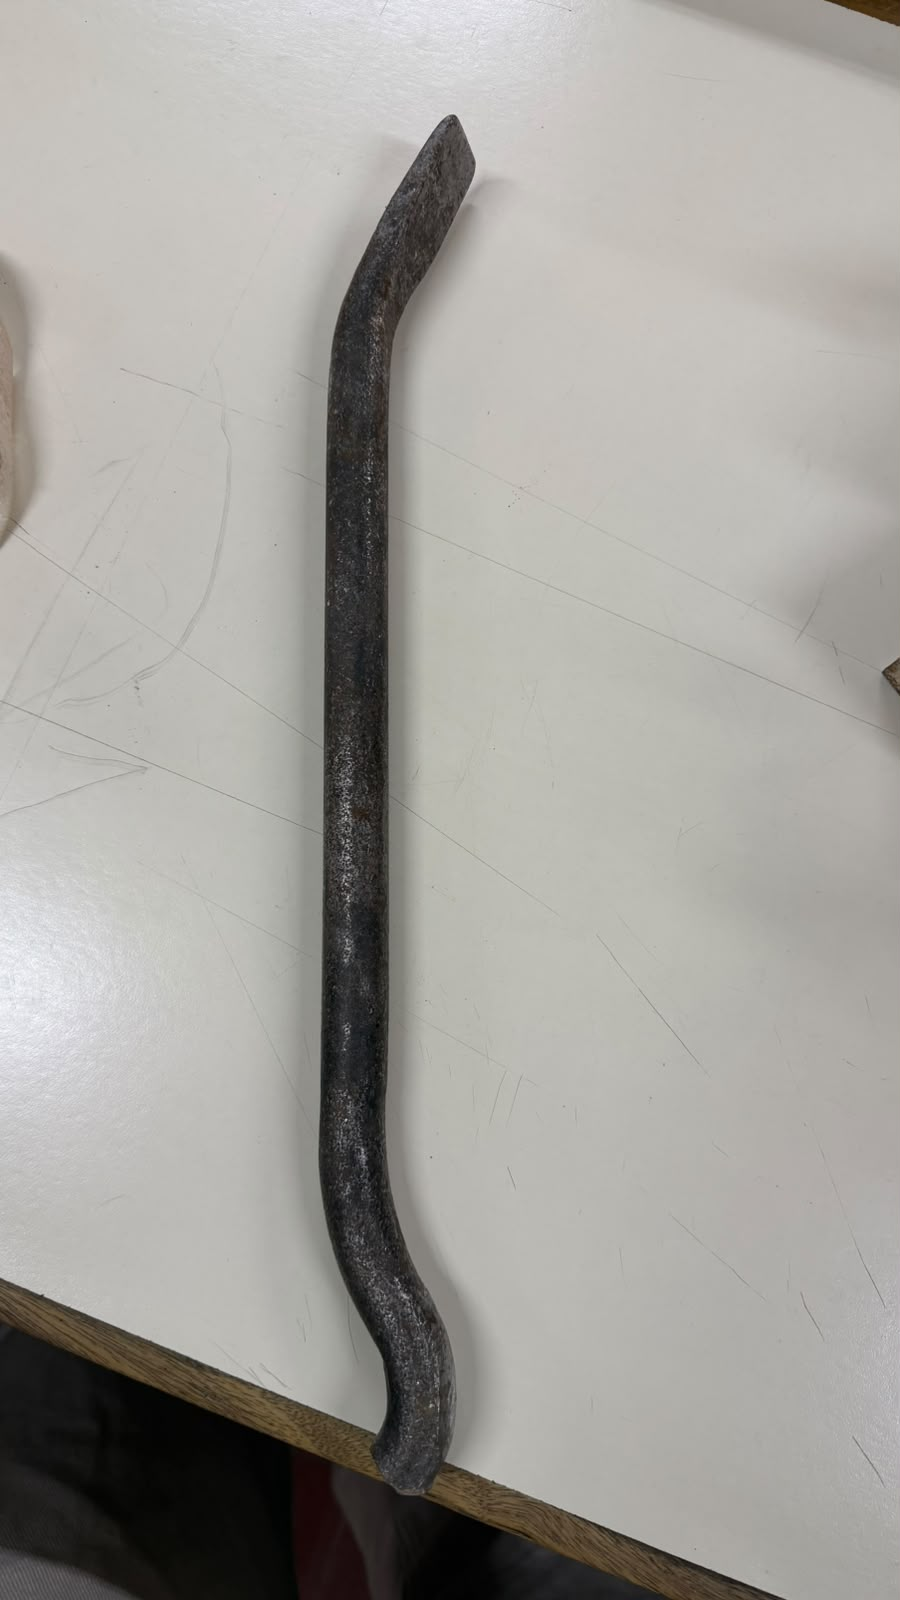
\includegraphics[height=1.85cm]{foto1.jpg}} & Perfil general & 67 & 75 & 5--220 & $+2{,}8$ & 11 & 5{,}5\,\% & Completa; gancho sobre el borde de la mesa & Bolso, borde de mesa, piso, marcas de lápiz & No / No & Aceptable para análisis; no publicable\\
\addlinespace
2 & \raisebox{-.85\height}{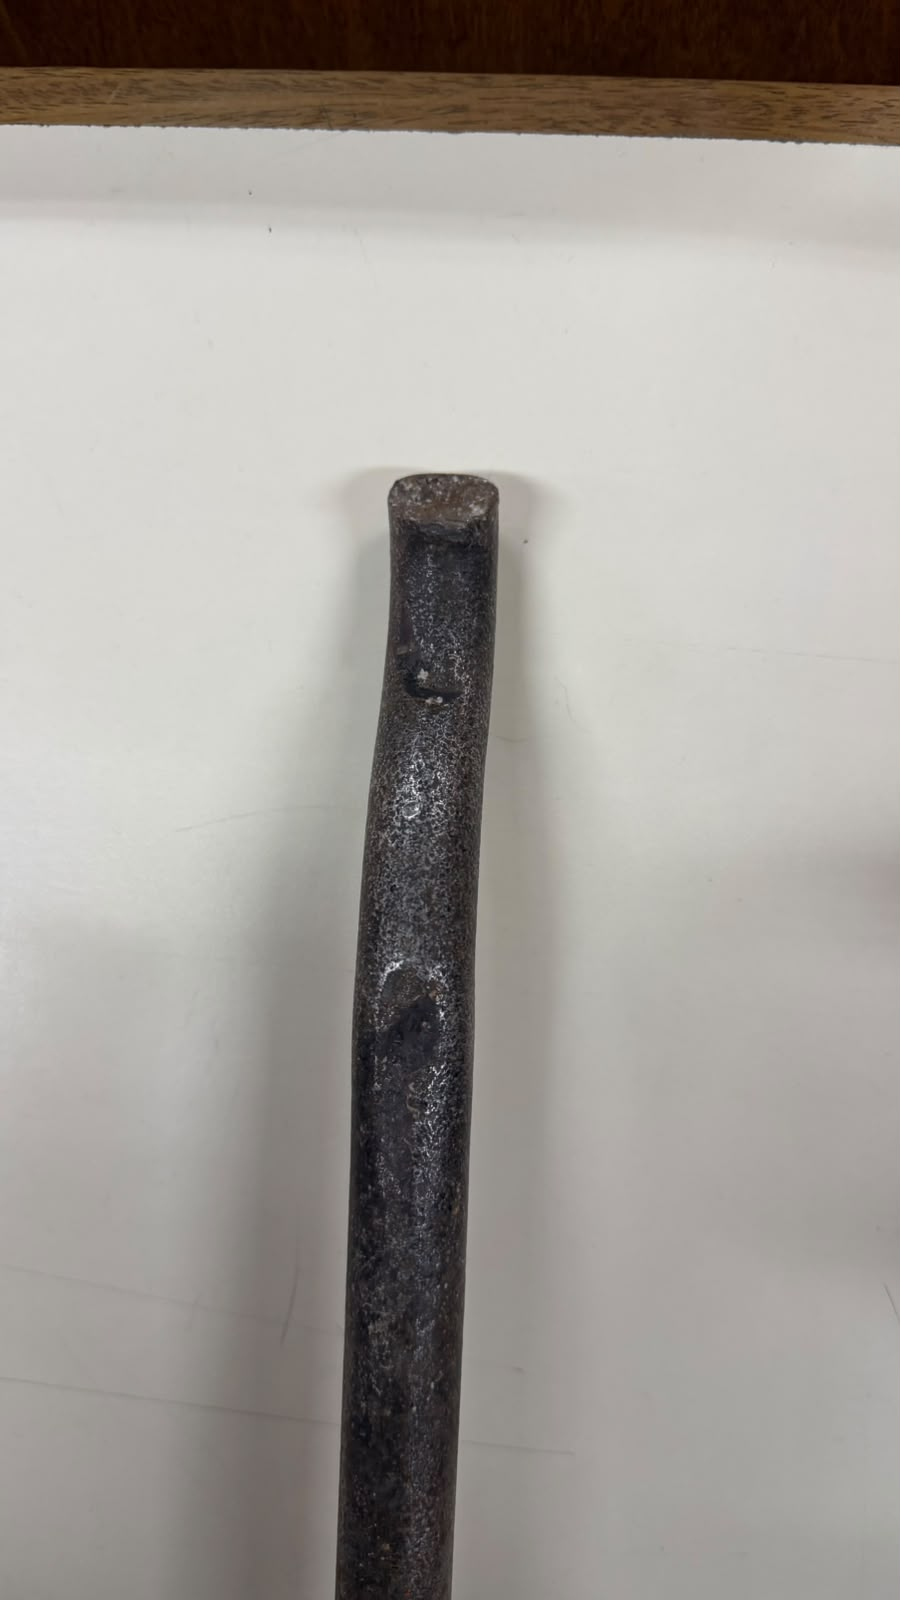
\includegraphics[height=1.85cm]{foto2.jpg}} & Detalle extremo superior & 63 & 76 & 15--217 & $+2{,}7$ & 21 & detalle & Correcto para un detalle & Borde de mesa y sombra arriba & No / No & Aceptable; repetir con luz rasante\\
\addlinespace
3 & \raisebox{-.85\height}{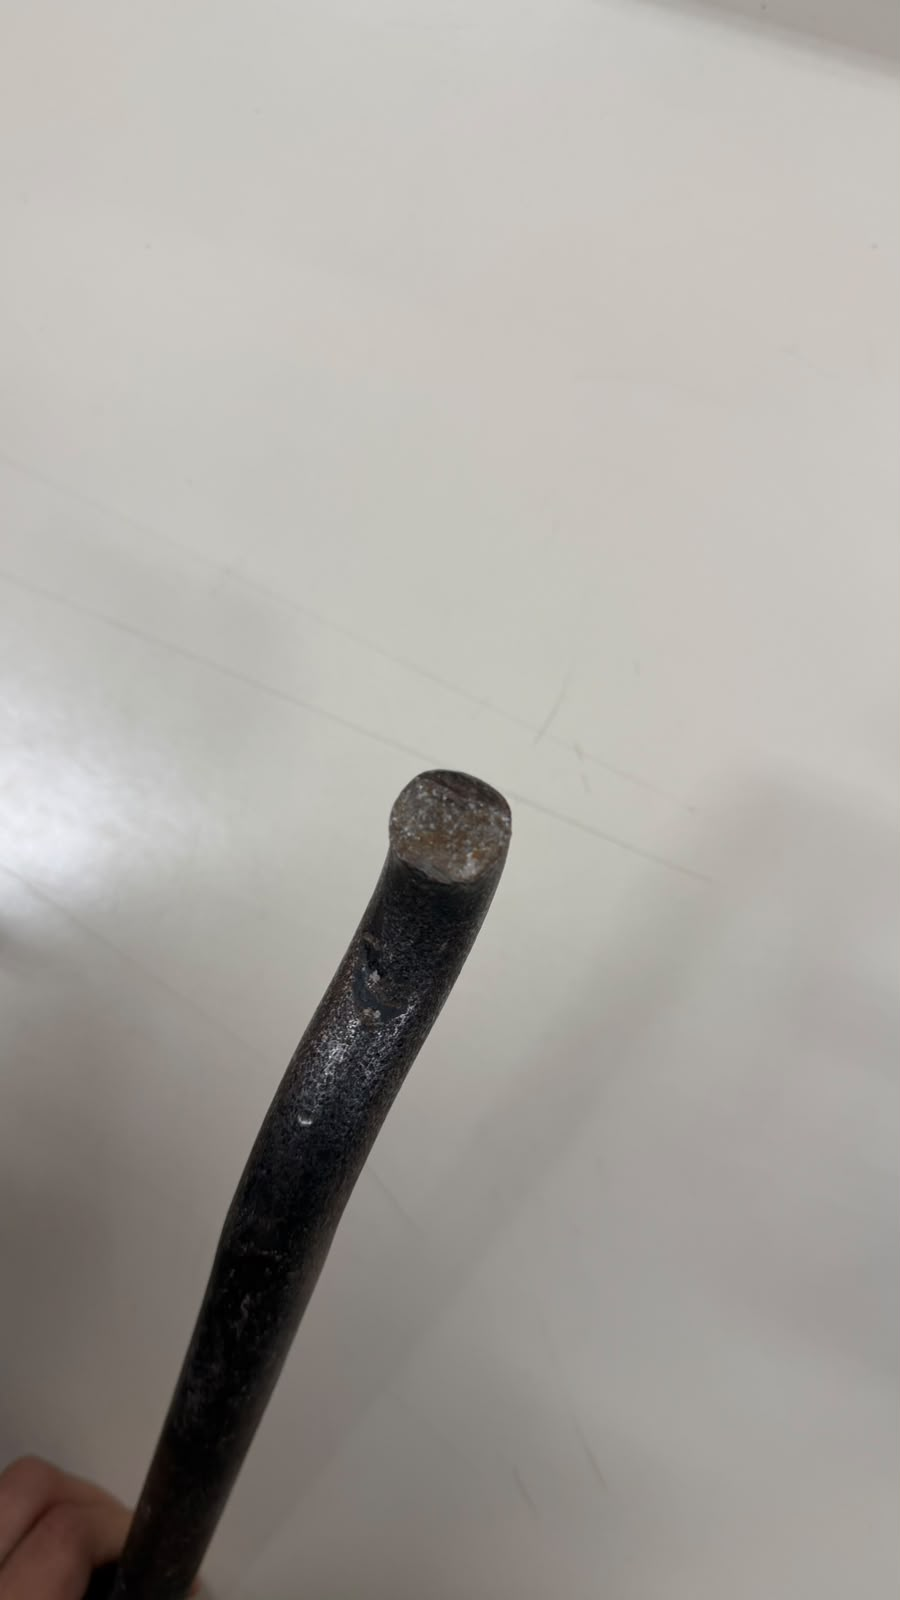
\includegraphics[height=1.85cm]{foto3.jpg}} & Sección transversal & 20 & 76 & 6--210 & $+3{,}1$ & 16 & detalle & Pieza en diagonal; fondo vacío arriba & Mano, reflejo en la mesa & No / No & Desenfocada: repetir\\
\addlinespace
4 & \raisebox{-.85\height}{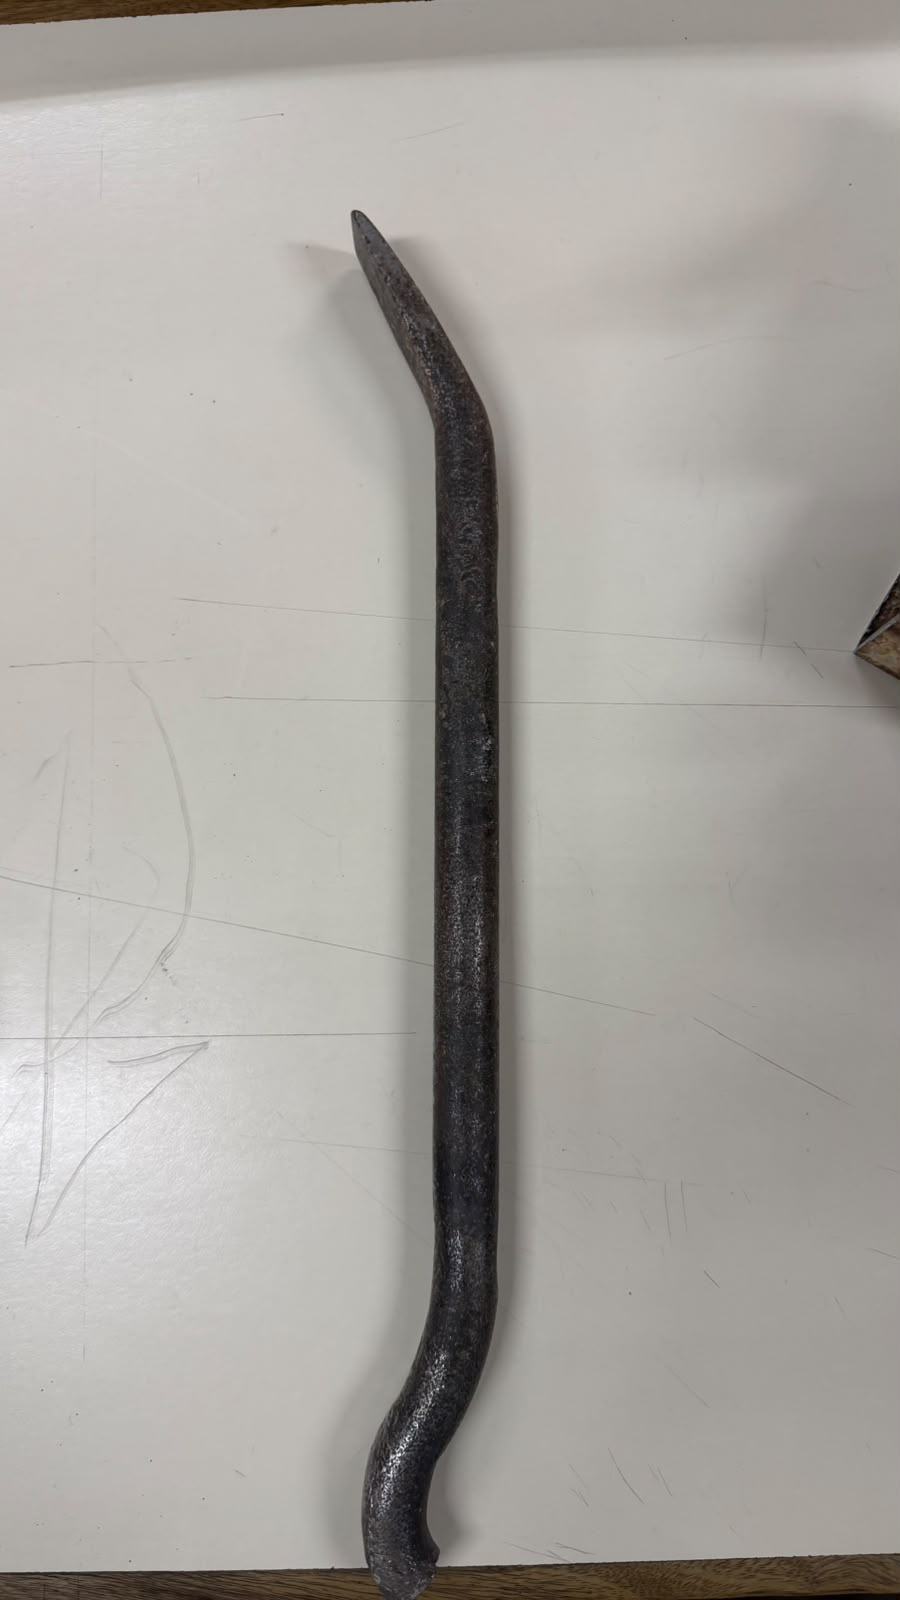
\includegraphics[height=1.85cm]{foto4.jpg}} & Longitudinal completa & 62 & 73 & 32--222 & $+3{,}0$ & 19 & 6{,}3\,\% & Extremo inferior a 35\,px del borde & Objeto a la derecha, borde de mesa & No / No & Aceptable para análisis; no publicable\\
\addlinespace
5 & \raisebox{-.85\height}{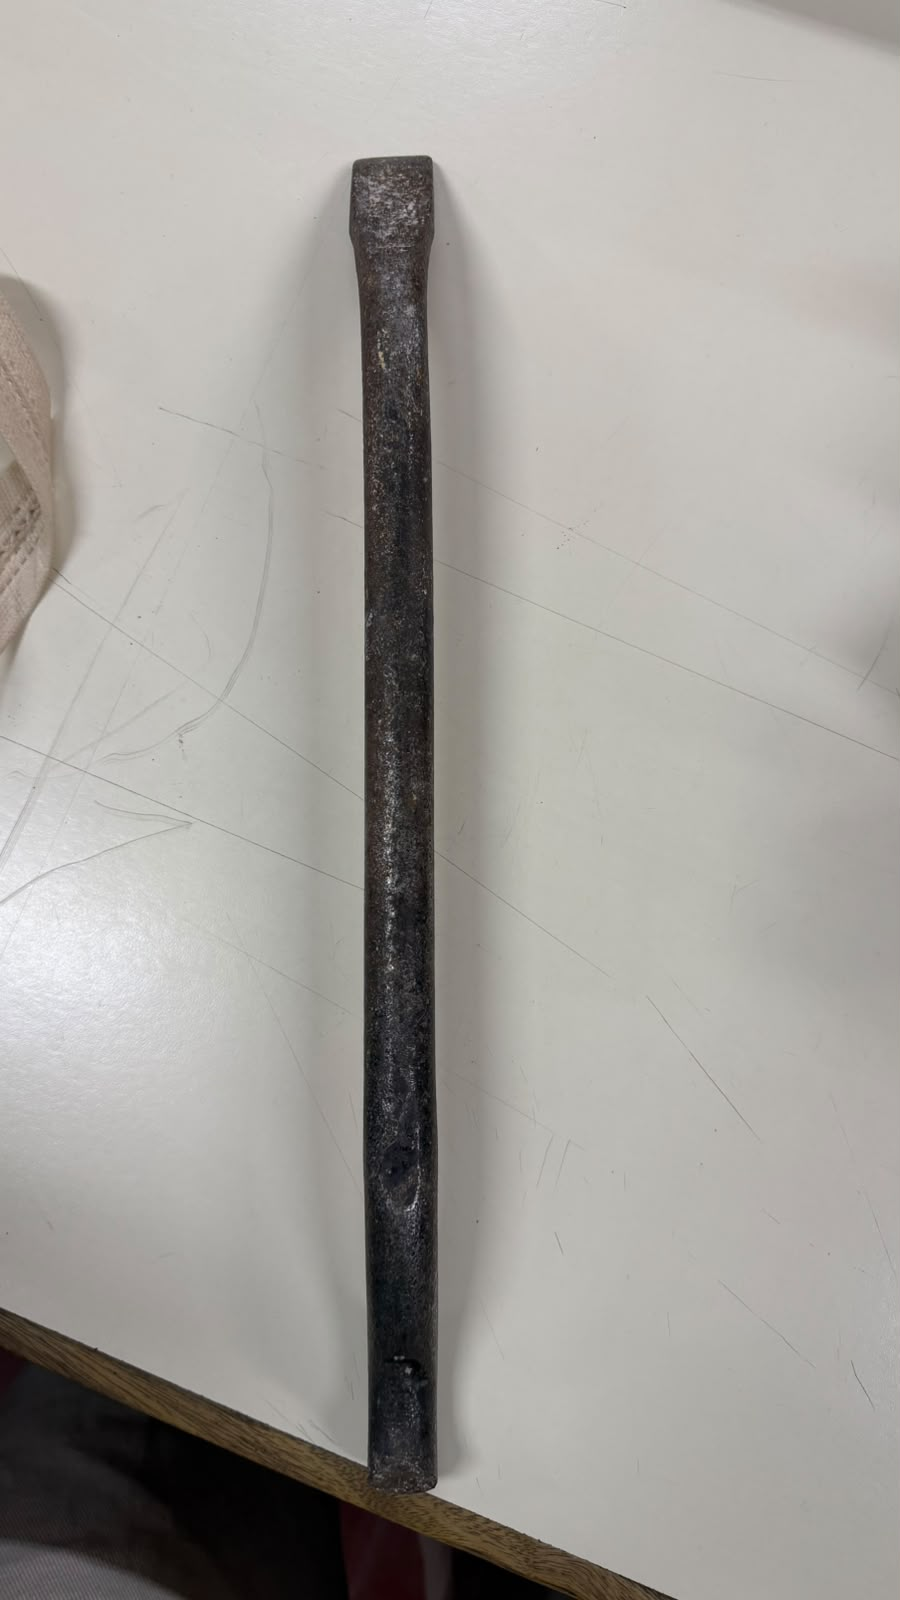
\includegraphics[height=1.85cm]{foto5.jpg}} & Posterior / alineación & 65 & 75 & 4--223 & $+2{,}8$ & 16 & 6{,}0\,\% & Completa y centrada & Bolso, borde de mesa, piso & No / No & La mejor de la serie; falta escala\\
\midrule
\multicolumn{3}{l}{\textbf{Referencia deseable}} & $>50$ & 90--95 & 5--250 & $\approx0$ & $<5$ & $>$30\,\% & Completa con margen & Ninguno & Sí / Sí & \\
\bottomrule
\end{tabular}

\medskip
\begin{minipage}{0.95\linewidth}\footnotesize
Nitidez: varianza del laplaciano. $L^*$: luminosidad media del fondo (0 = negro, 100 = blanco). Rango: percentiles 1 y 99 del nivel de gris (0--255). $b^*>0$: dominante amarilla. $\Delta L^*$: diferencia de luminosidad del fondo entre la zona más clara y la más oscura de una grilla de $4\times4$. Ocupación: porcentaje del área de la imagen cubierto por la pieza. Resolución de todas las tomas: $900\times1600$\,px, sin metadatos EXIF. Ninguna toma tiene píxeles saturados en blanco (menos del 0{,}01\,\%).
\end{minipage}
\end{table}
\end{landscape}

\begin{figure}
\centering
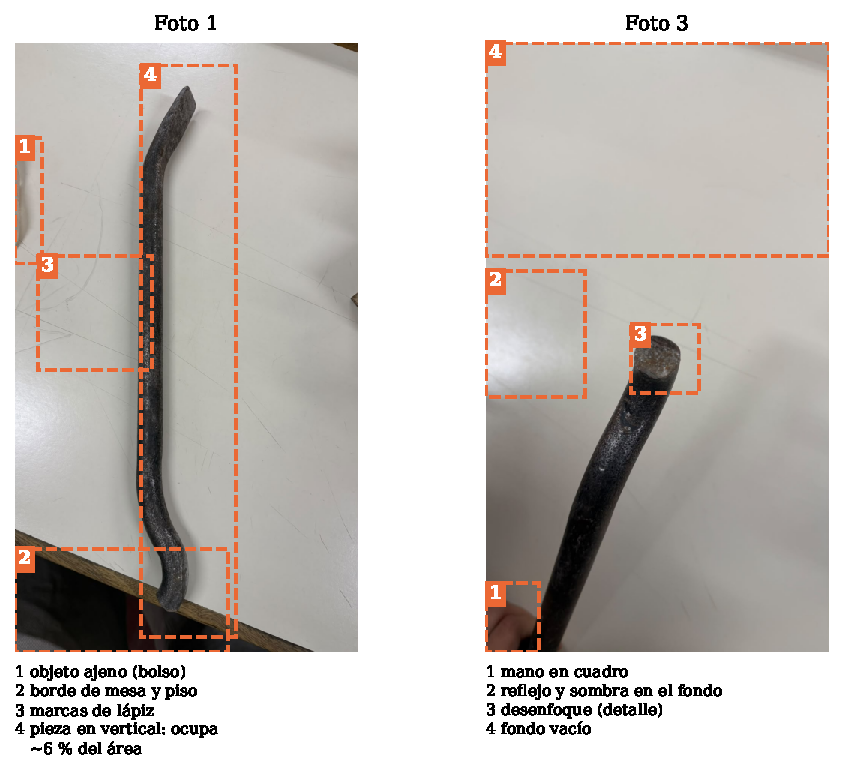
\includegraphics[width=\textwidth]{problemas.pdf}
\caption{Problemas detectados en las Fotos 1 y 3. Los recuadros numerados corresponden a la lista bajo cada imagen.}
\label{fig:problemas}
\end{figure}

\subsection{Lo que está bien}

\begin{itemize}
\item \textbf{Fondo claro y liso.} El fondo ocupa entre el 73 y el 83\,\% de cada imagen y contrasta con el acero oscuro, lo que permite leer el contorno de la pieza y separarla automáticamente del fondo.
\item \textbf{Sin luces quemadas.} Menos del 0{,}01\,\% de los píxeles está saturado en blanco, así que no se perdió información en las zonas claras. No se usó flash, que en el acero produce reflejos fuertes.
\item \textbf{Balance de blancos casi neutro.} El fondo tiene $a^*\approx0$ y $b^*\approx+3$: hay una leve dominante cálida, pero los colores del óxido y del acero se ven naturales.
\item \textbf{Nitidez.} Cuatro de las cinco tomas tienen una nitidez adecuada (62 a 67).
\item \textbf{Secuencia ordenada.} Se fue de lo general a lo particular y se incluyó una vista a $90^\circ$ (Foto 5), que permite evaluar la alineación del eje desde otro plano \cite{forense}.
\item \textbf{Tomas comparables.} Las vistas generales tienen orientación y distancia parecidas, lo que facilita compararlas entre sí.
\end{itemize}

\subsection{Lo que se debe mejorar}

\begin{itemize}
\item \textbf{Exposición.} El fondo blanco tiene $L^*\approx75$ cuando debería estar cerca de 90--95, por lo que se ve gris. El fotómetro del celular promedia la escena y, como la mesa blanca ocupa casi toda la imagen, la subexpone. Además, el percentil 99 no supera 223, así que no se usa la parte alta del rango tonal. \emph{Solución:} compensar la exposición en $+2/3$ a $+1$\,EV, o medir la luz sobre una tarjeta gris.
\item \textbf{Iluminación despareja.} La luminosidad del fondo varía entre 11 y 21 unidades de $L^*$ dentro de una misma imagen, por sombras y por la luz de ventana o de techo. \emph{Solución:} dos fuentes difusas iguales a $45^\circ$ de cada lado para las vistas generales y luz rasante (casi paralela a la superficie) solo para las tomas de detalle de golpes y textura.
\item \textbf{Encuadre.} La pieza, larga y delgada, se fotografió en vertical y ocupa apenas el 6\,\% del área; el resto es fondo. En la Foto 4 el extremo inferior queda a 35 píxeles del borde. \emph{Solución:} ubicar la pieza en horizontal o en diagonal según la forma del cuadro, llenar al menos un tercio de la imagen y dejar un margen parejo alrededor.
\item \textbf{Objetos y marcas ajenas.} Aparecen un bolso, el borde de la mesa, el piso, otro objeto, una mano y marcas de lápiz sobre la mesa. Distraen y, en un peritaje, pueden generar dudas sobre qué es evidencia. \emph{Solución:} usar un fondo de papel o cartulina blanca (o gris neutro) que cubra todo el cuadro y despejar la zona.
\item \textbf{Sin escala ni rótulo.} No hay testigo métrico ni identificación de caso, fecha y pieza, por lo que no se pueden dar medidas absolutas ni vincular la foto con la pieza. \emph{Solución:} regla o escala forense en el mismo plano que la pieza y un rótulo con número de caso, fecha y número de toma.
\item \textbf{Perspectiva.} La cámara no estuvo perpendicular a la mesa: el ancho aparente de la barra varía entre tomas y los bordes de la mesa no son paralelos al cuadro. \emph{Solución:} trípode o soporte, y nivel en el celular.
\item \textbf{Desenfoque.} La Foto 3 tiene una nitidez de 20, tres veces menor que las demás, y es justamente una toma de detalle. \emph{Solución:} tocar la pantalla sobre la pieza para enfocar, apoyar el celular y revisar cada toma ampliada antes de seguir.
\item \textbf{Resolución.} Las copias tienen $900\times1600$ píxeles porque se reenviaron por mensajería, que reduce la imagen. A 300\,ppp, el mínimo habitual para fotografías impresas \cite{allen}, el lado menor solo alcanza para una figura de 7{,}6\,cm de ancho; el ancho completo de una página LNCS (12{,}2\,cm) necesita 1441 píxeles. \emph{Solución:} usar los archivos originales del celular, que tienen varias veces más píxeles.
\item \textbf{Integridad.} Las copias no conservan los metadatos EXIF (fecha, hora y equipo). \emph{Solución:} descargar los originales por cable o desde la nube sin compresión, calcular su huella SHA-256 el mismo día y trabajar siempre sobre copias \cite{astm860}.
\end{itemize}

\section{Preparación de una imagen para publicación}

Para publicar, una fotografía puede recibir \emph{ajustes globales}, es decir, aplicados por igual a toda la imagen: recorte, rotación, brillo, contraste y balance de blancos. No se puede borrar, agregar ni mover nada dentro de la imagen, ni retocar una zona en particular. Todo ajuste debe declararse y el original debe conservarse \cite{rossner}.

La Fig.~\ref{fig:antesdespues} muestra la Foto 1 preparada con esos ajustes: se rotó $90^\circ$ para aprovechar el ancho de la página, se recortó a la zona de la pieza y se escaló cada canal de color para que el fondo quede blanco y neutro. El resultado es más legible, pero sigue mostrando los límites que no se corrigen después: la sombra, el borde de la mesa y la falta de escala. Esos problemas solo se resuelven al momento de la toma.

\begin{figure}
\centering
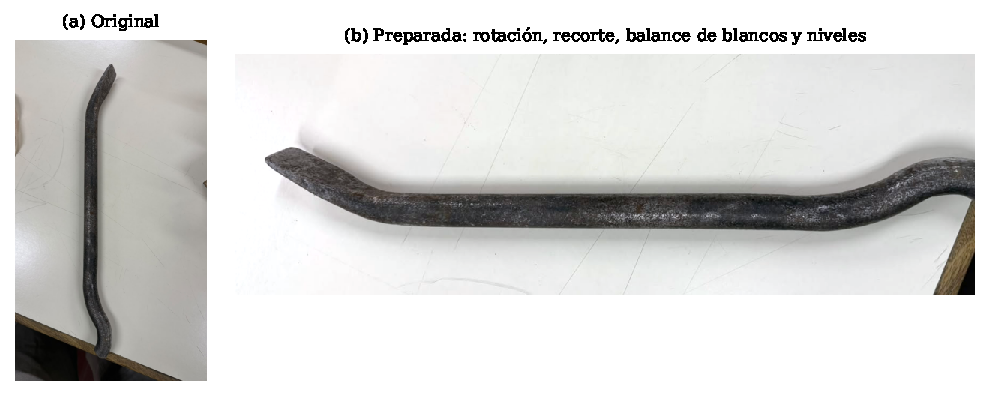
\includegraphics[width=\textwidth]{antes_despues.pdf}
\caption{Foto 1 original (a) y preparada para publicación (b) solo con ajustes globales.}
\label{fig:antesdespues}
\end{figure}

\section{Protocolo recomendado}

A partir de lo anterior se propone el siguiente protocolo para futuras tomas:

\begin{enumerate}
\item \textbf{Preparar la escena:} fondo continuo blanco o gris neutro, sin otros objetos; dos luces difusas a $45^\circ$.
\item \textbf{Ubicar referencias:} escala forense en el plano de la pieza, rótulo con caso, fecha y número de toma, y una tarjeta gris o carta de color en la primera toma.
\item \textbf{Fijar la cámara:} trípode o soporte, cámara perpendicular a la pieza (verificar con nivel), sin zoom digital.
\item \textbf{Exponer y enfocar:} compensar la exposición para que el fondo se vea blanco sin quemarse; enfocar sobre la pieza; no usar flash directo.
\item \textbf{Encuadrar:} pieza completa, orientada según el formato, ocupando al menos un tercio de la imagen y con margen parejo.
\item \textbf{Tomar la serie:} vistas generales de todas las caras, vistas a $90^\circ$, y detalles con luz rasante.
\item \textbf{Verificar en el momento:} ampliar cada toma para comprobar el foco antes de mover la pieza.
\item \textbf{Resguardar:} descargar los originales sin compresión, nombrarlos de forma ordenada (caso\_fecha\_toma), calcular su SHA-256 y trabajar sobre copias.
\end{enumerate}

\section{Conclusiones}

Las fotografías del taller cumplieron su función principal: permitieron identificar el mecanismo de falla y hasta medir ángulos y rectitud sin escala. Sus fortalezas (fondo liso y contrastado, ausencia de luces quemadas, color casi neutro, buena nitidez y secuencia ordenada) muestran que con un celular se puede obtener material técnico útil.

Sin embargo, no alcanzarían la calidad de un artículo científico ni de un peritaje formal. Los problemas más importantes son la falta de escala y de rótulo, el encuadre con poca ocupación, los objetos ajenos, la exposición baja del fondo y la pérdida de resolución y metadatos al reenviar los archivos. Casi todos se resuelven al momento de la toma y no después, por lo que el protocolo propuesto apunta a preparar la escena antes de fotografiar.

\begin{credits}
\subsubsection{Uso de inteligencia artificial.} En la elaboración de este informe se utilizaron herramientas de IA generativa como asistentes de redacción y para programar las mediciones sobre las imágenes. Los resultados y las conclusiones fueron revisados por el equipo.
\end{credits}

\begin{thebibliography}{8}

\bibitem{allen}
Allen Press: Digital Art Support: Acceptable Resolutions. \url{https://www.allenpress.com/support/digital-art-support/}, último acceso: 13/11/2026

\bibitem{astm860}
ASTM International: ASTM E860-22, Standard Practice for Examining and Preparing Items That Are or May Become Involved in Criminal or Civil Litigation. ASTM International, West Conshohocken (2022)

\bibitem{gonzalez}
Gonzalez, R.C., Woods, R.E.: Digital Image Processing, 4th edn. Pearson, New York (2018)

\bibitem{forense}
Kemelmajer, S., Martinez, R.A., Mujica, M.P., Salamone, L.: Taller de Fotografía Forense Digital: análisis de falla de una palanqueta de acero. Informe del Módulo 2, Técnicas y Herramientas Modernas, Universidad Nacional de Cuyo (2026)

\bibitem{rossner}
Rossner, M., Yamada, K.M.: What's in a picture? The temptation of image manipulation. Journal of Cell Biology \textbf{166}(1), 11--15 (2004)

\end{thebibliography}

\end{document}
